\documentclass[12pt]{article}
\usepackage[a4paper, margin=1.5in]{geometry}
\setlength{\headheight}{15pt}
\usepackage[utf8]{inputenc}
\usepackage{graphicx}\graphicspath{{figures/}}
\usepackage{authblk}
\renewcommand*{\Authsep}{, }
\renewcommand*{\Authand}{\\ \bigskip}
\renewcommand*{\Authands}{\\ \bigskip}
\setlength{\parindent}{0pt} % disables indentation
\usepackage{multicol}
\usepackage{enumitem}
%%%%%%%%%%%%%%%%%%%%%%%%%%%%%%%%%%%%%
\usepackage{fancyhdr}\pagestyle{fancy}
\fancyhf{}
\fancyhead[R]{\thepage}
\fancyfoot{}
% \usepackage{emptypage}
\usepackage[hidelinks]{hyperref}
%%%%%%%%%%%%%%%%%%%%%%%%%%%%%%%%%%%%
\usepackage{tikz}
\usetikzlibrary{arrows}
\usetikzlibrary{shapes.geometric}
%%%%%%%%%%%%%%%%%%%%%%%%%%%%%%%%
% FOR FLOW CHART DECLARATION
\tikzstyle{startstop} = [ellipse,  minimum width=3cm, minimum height=1cm,text centered, draw=black, fill=red!30]
\tikzstyle{io} = [trapezium, trapezium left angle=70, trapezium right angle=110, minimum width=3cm, minimum height=1cm, text centered, draw=black, fill=blue!30]
\tikzstyle{process} = [rectangle, minimum width=3cm, minimum height=1cm, text centered, draw=black, fill=orange!30]
\tikzstyle{decision} = [diamond, aspect=4, minimum width=3cm, minimum height=1cm, text centered, draw=black, fill=green!30]
\tikzstyle{arrow} = [thick,->,>=stealth]
%%%%%%%%%%%%%%%%%%%%%%%%%%%%%%%%%%%%
\title{
    
\includegraphics[scale = 0.6]{BUET_logo.pdf} \\
    \bigskip \Large{CSE 316\\ Microprocessors, Microcontrollers, and Embedded Systems Sessional : Term Project} \\
    \Huge{Tetris}
    \bigskip
}
\author[]{Asif Ajrof (1705092)}
\author[]{Fatima Nawmi (1705093)} 
\author[]{Supervised by \\ Md. Masum Mushfiq \\ Lecturer}
\affil[]{Department of Computer Science and Engineering, \\ Bangladesh University of Engineering and Technology}
\date{July 2021}

\begin{document}
\maketitle
\thispagestyle{empty}
\newpage

\pagenumbering{roman}
\pagestyle{plain}
\tableofcontents
\newpage

\pagenumbering{arabic}
\pagestyle{fancy}
\section{Motivation}
    Remaking the popular arcade game Tetris in a simple platform using microcontroller and LED matrices.

\section{Components}
    The main components of our project are:
    \begin{enumerate}
        \item ATmega32
        \item 8x8 LED Dot Matrix (common cathode)
        \item 16x2 LCD Screen
        \item Thumb Joystick
        \item Buzzer 
    \end{enumerate}

    Some other components that were also used:
     \begin{multicols}{3}
        \begin{itemize}
            \item USBasp
            \item Resistor
            \item Inductor
            \item Capacitor
            \item Wire
            \item Potentiometer
        \end{itemize}
    \end{multicols}

\section{Short Description of Each Module}
    We have several different modules in this project. Here is a short description summarizing what each module does individually.
    
    \subsection{Main Console}
        The main gaming console is made of two 8x8 LED Dot Matrix, so we have a 16x8 display for the gameplay.

    \subsection{Pieces}
        We have kept all the 7 different pieces of Tetris game (I,J,L,T,S,Z,O). The pieces are generated randomly, and for each game the pieces are random as well.\vspace{1em}
        
        We show the next piece to come in the LCD screen.For this we have ensured communication between two ATmega32.
    
    \subsection{Movement}
        The thumb joystick is used for four possible movements: left, right, down and rotate (up move of joystick). Also, for starting the game we need an up move.

    \subsection{Score Update}
        When a row is filled the score is updated in the LCD screen and the filled row is removed while the rows above come down to fill up the empty row. When four consecutive rows are filled at the same time, as a bonus double points are added.
    
    \subsection{Game Speed}
        After certain time intervals, the game increases its speed. The speed resets when a new game is started again.
        
    \subsection{Sound}
        The buzzer makes a sound when there is a score update, a new game starting and when the game is over.

    \subsection{Game over and New game}
        When there is no more place for a new piece to enter, the game is over. 

        For a new game to begin after the last game is over,the display shows a play button and an up movement is needed.
        
\section{Methods used}
    \subsection{UART}
        For having a simplex data transfer we used UART subsystem. We used 9600 bps baud rate for data transmission.

    \subsection{ADC}
        We have used the ADC chip for collecting analogue movement data from the thumb joystick and converted it to digital for our piece movements.

\section{Algorithm used in gameplay}
    The algorithm used in gameplay is shown in the following flowchart,
    \begin{figure}[h!]
        \centering
        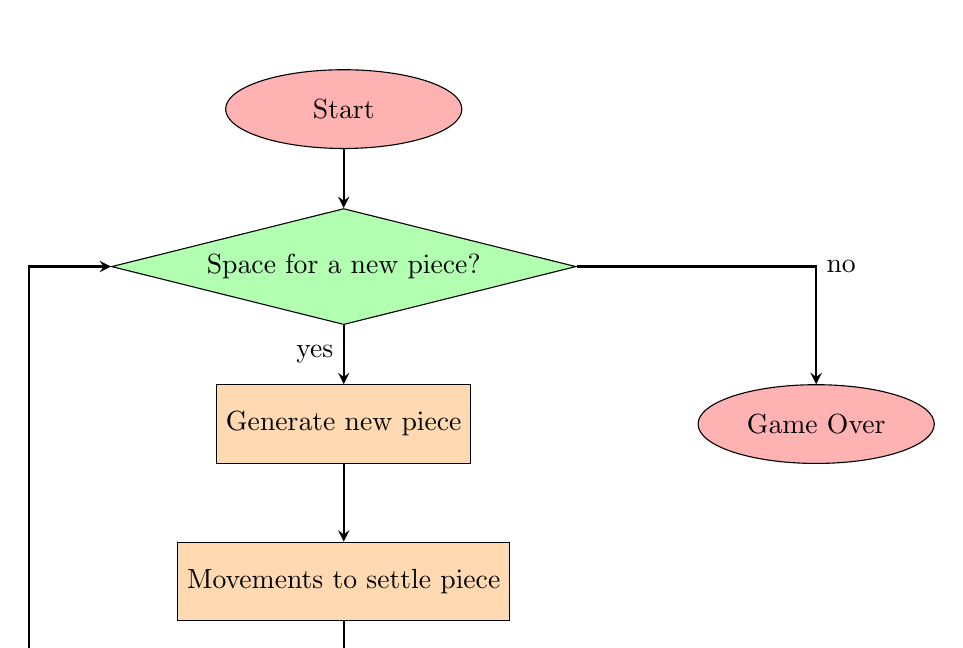
\begin{tikzpicture}
            \node[startstop] (start) {Start}; 
            \node[decision, below of = start, yshift=-1cm] (dec1) {Space for a new piece?};
            \node[process, below of = dec1, yshift=-1cm] (p1) {Generate new piece};
            \node[startstop, right of = dec1, xshift = 5 cm, yshift = -2cm ] (p2) {Game Over};
            \node[process, below of = p1, yshift=-1cm] (p3) {Movements to settle piece};
            \draw[arrow] (start) -- (dec1);
            \draw[arrow] (dec1) -- node[left] {yes} (p1);
            \draw[arrow] (dec1) -| node[right] {no} (p2);
            \draw[arrow] (p1) -- (p3);
            \draw[thick](p3) -- (0,-7);
            \draw[thick](0,-7) -- (-4,-7);
            \draw[arrow](-4,-7) |- (dec1);
        \end{tikzpicture}
        \caption{Algorithm}
        \label{fig:algo}
    \end{figure}

\section{Circuit Diagram}
    \begin{figure}[ht]
        \centering
        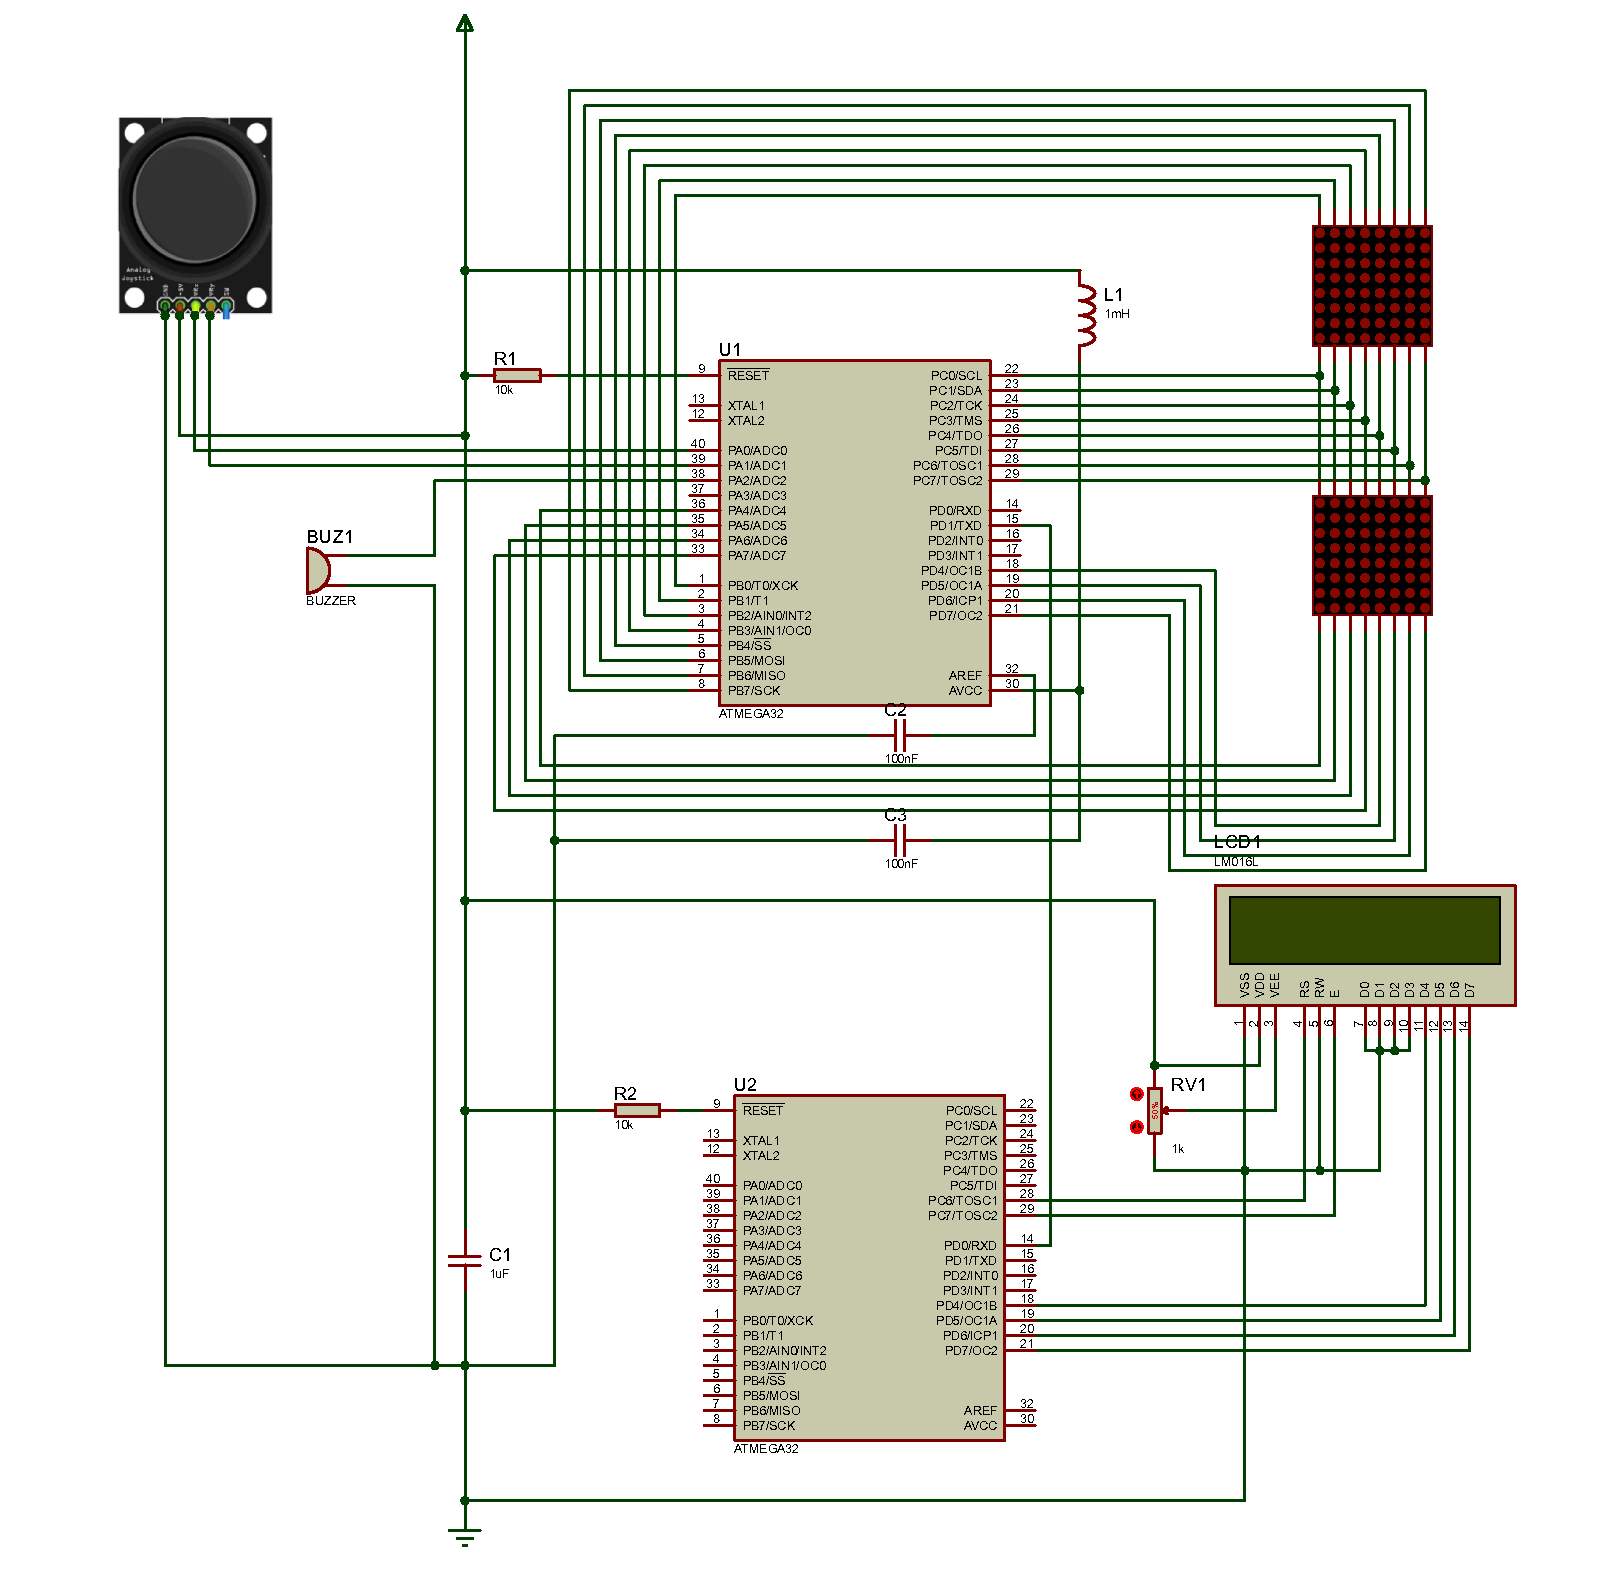
\includegraphics[width = \textwidth]{circuit_final1.pdf}
        \caption{Detailed Pin Diagram}
        \label{fig:circuit}
    \end{figure}
    \begin{itemize}[leftmargin=*]
    \setlength\itemsep{-0.1em}
        \item We have used two ATmega32 microcontrollers, $U1$ and $U2$ in the Figure \ref{fig:circuit}.%\vspace{0.5em}
        
        \item The main console, i.e., two LED dot matrices are connected to $U1$. Since we have used two common cathode LED matrices, we have used $PORTC$ for the common row connection for both LED matrices. For column connection we have connected the upper LED matrix to $PORTB$ and the lower LED matrix to $PA4-PA7$ and $PD4-PD7$.%\vspace{0.5em}
    
        \item As we have connected the thumb joystick using the $ADC0,ADC1$ input, it is connected to $PA0-PA1$, also the ground pin of the joystick is connected to the common ground of the circuit and the power pin to the common power source, $VCC$. We have used $AVCC$ as the voltage source for ADC and for better accuracy and stable voltage we have connected a capacitor ($C2$) between ground and $AREF$, another one ($C3$) between ground and $AVCC$. For stable current flow we have used an inductor ($L1$) between $AVCC$ and $VCC$.%\vspace{0.5em}
    
        \item We have connected the positive end of the the buzzer to $PA2$ and the negative end to the ground.%\vspace{0.5em}
        
        \item For establishing $UART$ serial communication between $U1$ and $U2$ we have connected the TXD ($PD1$) pin of $U1$ to the RXD ($PD0$) pin of $U2$.%\vspace{0.5em}
    
        \item We have connected the LCD to $U2$, using $PD4-PD7$ as data lines $D4-D7$, and $PC6,PC7$ as register select and enable pins respectively. As we have used the LCD for only write operations, the Read/Write pin is constantly kept low by connecting it to the ground. Since we have used 4-Bit Mode Interfacing, data pins $D0-D3$ are connected to the ground. The $VEE$ pin is connected to a potentiometer for changing the contrast of the display. The $VDD$ pin is connected to power source and the $VSS$ pin is connected to the ground.%\vspace{0.5em}
    
        \item For ensuring stable source voltage we have used a capacitor between source voltage and ground in both $U1$ and $U2$ and the reset pin is connected to the $VCC$.
    \end{itemize}
   
\section{Challenges}
    \begin{itemize}[leftmargin=*]
        \item We noticed that while using UART serial communication the data transfer was delayed by few seconds, for fixing this we tried using a larger Baud rate for a larger bit per second, but after some trial and error even with a larger Baud rate there was some delay, hence when the score gets updated or game over or a new game there is a slight delay before the LCD is updated.

        \item We faced a problem in our main display LED matrices, every next row was emitting very dim light under the actual positions. We figured since we are multiplexing the rows and columns, and we are changing the row values first and then changing the column values, as a result for a very brief time the columns are getting previous values for an updated row value. We fixed this problem by clearing the values of columns after a short delay in each iteration.

        \item While implementing the movements a delay was needed because without delay a single press would trigger multiple moves. But a delay function for every movement pauses all the other functionalities. So, instead we kept a variable, that keeps count of the duration of one button press and ensures one movement for one press.

        \item While designing our main circuit we first wanted to use one ATmega32 with the help of decoders for all our operations. We tried simulating this with Proteus, but we noticed because of using decoder the entire process was becoming very slow. So we excluded this idea from the designing phase and designed with two ATmega32 which also enabled us to learn about the serial communication method.

        \item Even though we needed simplex serial communication between the two microcontrollers we found that if we did not enable the RXC and TXC of UCSRA registers in both ATmega32 code, it was not working in hardware, but it was working in simulation. Hence we used duplex mode for implementing simplex communication.

        \item LCD showed garbage values if there was a slight change in voltage, after reconnecting the voltage source this problem went away. For solving this issue we have called the LCD initialization function every time before we write something on the LCD. This clears the garbage values without the necessity to reset.

        \item Implementing all the logistics of the game into hardware was very challenging. Implementing the same tasks in simulator was widely different than implementing it in hardware.
    \end{itemize}

\end{document}